\documentclass[11pt,a4paper,fontset=fandol]{ctexart}
\usepackage[a4paper,margin=24mm,headheight=15pt]{geometry}
\usepackage{amsmath,amssymb,booktabs,tabularx,array,graphicx}
\usepackage{enumitem}
\usepackage{microtype}
\usepackage{xcolor}
\usepackage{hyperref}
\usepackage{fancyhdr}
\usepackage{natbib}

\hypersetup{
  colorlinks=true,
  linkcolor=blue!45!black,
  citecolor=green!35!black,
  urlcolor=blue!55!black,
  pdftitle={TerraState 中文完整审阅版},
  pdfauthor={Internal review copy}
}
\setlength{\parindent}{2em}
\setlength{\parskip}{0.35em}
\linespread{1.18}
\emergencystretch=3em
\setlist{nosep,leftmargin=2.2em}
\renewcommand{\arraystretch}{1.22}
\setlength{\tabcolsep}{4pt}
\newcolumntype{Y}{>{\raggedright\arraybackslash}X}

\pagestyle{fancy}
\fancyhf{}
\lhead{\small TerraState 中文完整审阅版}
\rhead{\small 非投稿文件}
\cfoot{\thepage}

\title{\bfseries TerraState：面向天气驱动地表预测的\\可检验预测状态世界模型}
\author{中文审阅版（英文 \texttt{paper/main.tex} 为唯一投稿事实源）}
\date{2026 年 7 月 28 日}

\begin{document}
\maketitle

\begin{quote}\small
本 PDF 用于作者审阅中文叙事、公式、表格与证据边界，不是 AAAI 投稿文件。
章节顺序、公式含义、实验数字与主张强度同步自英文权威稿。当前只展示已经接入
正式稿的 Figure 1；未批准的 Figure 2/3 不以空框或占位图出现。
\end{quote}

\tableofcontents
\clearpage
\addcontentsline{toc}{section}{摘要}
\begin{abstract}

高分辨率卫星预测能够利用受云遮挡的图像历史与气象驱动，支持植被和生态系统监测。然而，终点预测准确并不能证明模型形成了一个真正参与预测、并随声明天气驱动演化的内部状态。我们提出 \textbf{TerraState}：它从历史观测推断空间预测状态，使用共享的天气条件转移推进该状态，再将未来状态解码为最终预测中的显式贡献。训练期间，冻结的未来观测编码器为推进后的状态提供锚定，但不进入推理路径。我们将预测能力与同一个选定模型上的匹配干预分开评估。在 GreenEarthNet 时间偏移（OOD-t）划分上，TerraState 达到 $R^2=0.56935$、RMSE $=0.15059$。移除状态后，验证集和 OOD-t 上的官方 $R^2$ 分别下降 $0.01121$ 和 $0.01997$；对应配对效应均为正，95\% 置信区间分别为 $[0.00643,0.02590]$ 和 $[0.01422,0.03018]$。把真实未来天气替换为季节和地理匹配的 donor weather 或归一化均值天气后，终点损失分别增加 $0.00257$ 和 $0.01126$，两个置信区间均高于零。结果表明，TerraState 在保留有效预测能力的同时，暴露了一个真正承载预测、且预测行为依赖所提供未来天气的状态。

\end{abstract}

\section{引言}

高分辨率地球观测（Earth observation, EO）时间序列能够支持局地植被与生态系统响应监测，但提供的是部分观测：光学影像稀疏且经常受云遮挡，而地表演化还受到天气和静态地理条件影响。因此，从不完整历史和未来气象驱动预测未来地表观测，本质上是一个部分可观测的世界建模问题。模型需要从已有观测中推断预测状态，在外生驱动下推进该状态，再把状态映射回未来可观测量。EarthNet2021 将任务定义为由过去 Sentinel-2 观测、地形和未来气象共同引导的视频预测 \cite{requenamesa2021earthnet}；GreenEarthNet 随后引入面向植被的云掩膜、时间分布偏移评测和天气条件高分辨率预测器 \cite{benson2024multimodal}。

现有进展主要以固定时域的输出精度衡量。精度对于有用的世界模型是必要条件，却不能证明某个内部状态确实参与了预测。较低像素误差可能来自绕开所声明状态的预测路径，也可能来自对未来气象使用很弱的模型；准确预测还可能对应时间结构混乱的潜在表示 \cite{yang2026latenttsf}。由此产生本文的结构性问题：\textbf{一个准确的预测器是否真的暴露了由未来天气推进、并参与最终预测的状态？}

TerraState 通过把世界状态主张转化为可直接检验的模型性质来回应这一缺口。本文所称的预测状态，是从部分历史中推断、由共享转移在声明的未来驱动下推进、并能够重新映射为可观测预测的表示。要使这个状态在经验上有意义，其预测贡献必须能够在不重训练时被移除，而且真实未来天气应当比冻结天气对照产生更忠实的终点预测。这个定义比完整物理状态或因果模拟器更窄。它补充了输出层响应分析 \cite{luo2026eowm} 和场景条件潜状态滚动 \cite{iele2026vegsim}：本文追问的是暴露状态本身是否真正贡献于预测。

如 Figure 1 所示，TerraState 在一个预测模型中实现上述定义。历史编码器联合云掩膜 EO 历史、过去气象观测和静态地理，同时产生仅上下文预测与空间预测状态。一个共享转移在未来天气、地理和预测时距条件下推进状态；状态读出随后在仅上下文预测之外，对最终输出提供显式贡献。训练期间，真实未来观测的冻结表示用于锚定推进后的状态，但不进入推理。评测与这个结构逐项对应：Q1 衡量预测能力，Q2 移除状态贡献以检验它是否承载预测，Q3 替换未来天气以检验转移是否沿正确预测方向使用所提供的驱动。

GreenEarthNet 实验表明，TerraState 在时间偏移下保留了有效预测能力。在同一个选定模型上，移除状态贡献会在验证集和 OOD-t 上产生为正且置信区间不跨零的配对预测损失；真实天气也比 matched-donor weather 和归一化均值天气更忠实地预测终点。

本文贡献如下：

\begin{enumerate}
\item 我们将天气驱动的高分辨率地表预测表述为可检验的预测状态世界建模：由历史推断的空间状态经过一个共享的天气条件转移推进，并显式贡献于可观测预测。
\item 训练期间使用真实未来观测的冻结表示锚定推进后的状态，使未来观测监督作用于推理时仍位于预测路径中的状态。
\item 通过匹配证据链评测所得模型：时间偏移下的有效预测能力、验证集和 OOD-t 上承载预测的状态贡献，以及真实天气相较两个冻结天气对照更忠实的终点预测。
\end{enumerate}


\begin{figure}[htbp]
\centering
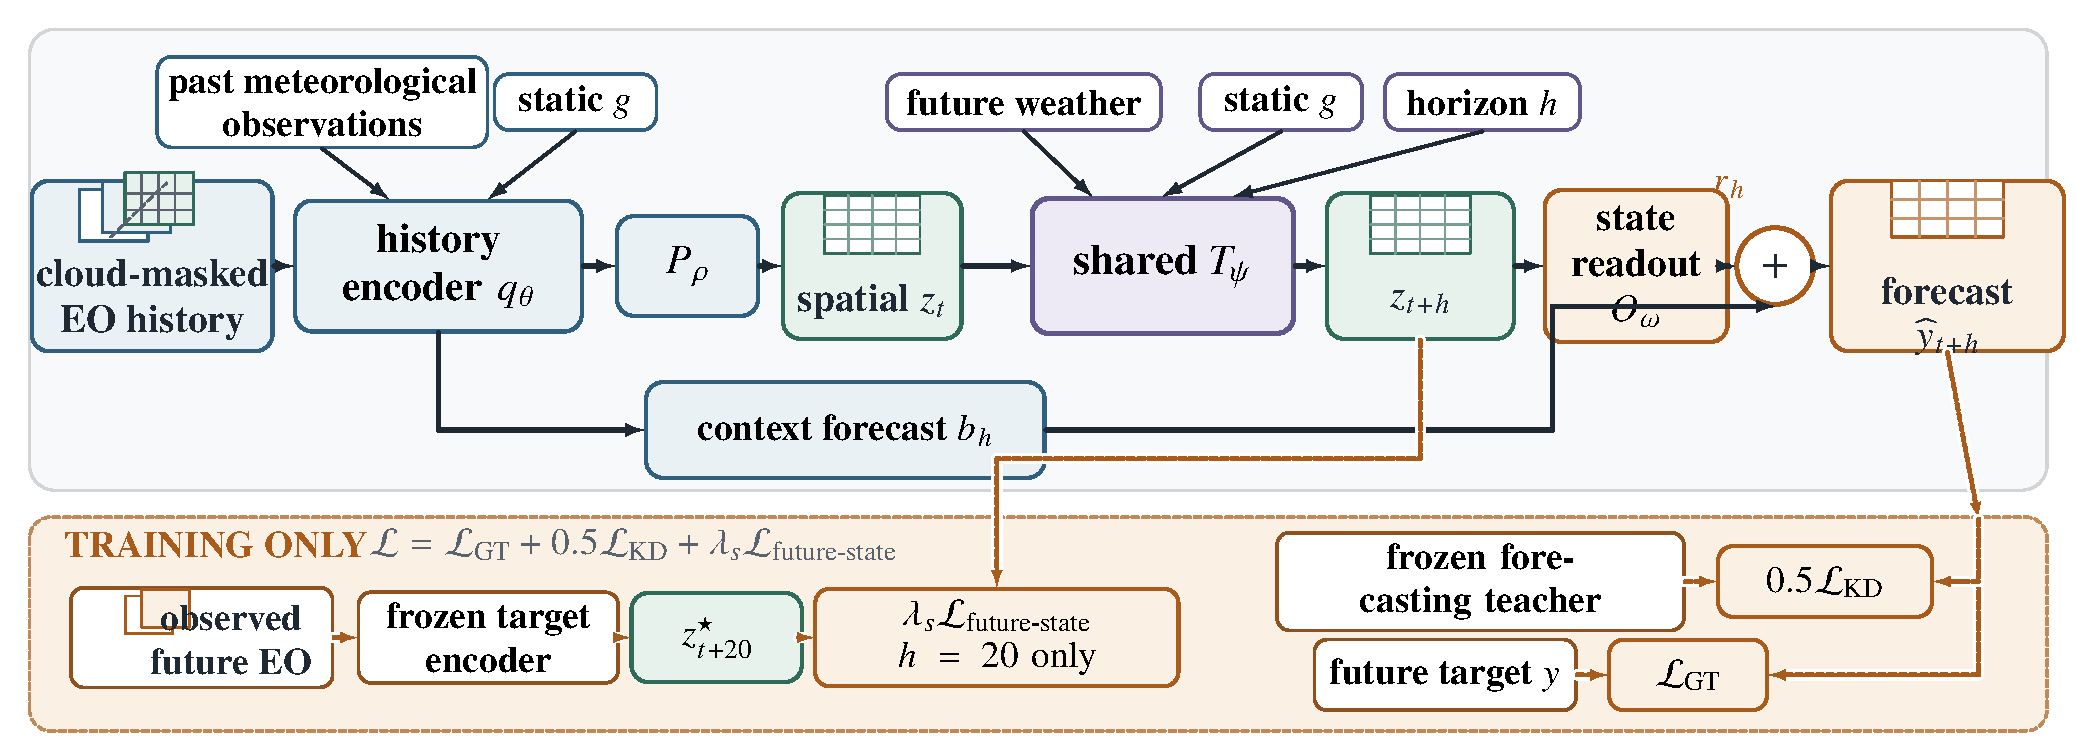
\includegraphics[width=\textwidth]{../paper/figures/terrastate_method_overview.pdf}
\caption{TerraState 推理路径与训练监督}
\end{figure}

\begin{quote}\small
可编辑矢量版本： \href{../paper/figures/terrastate\_method\_overview.pdf}{\texttt{terrastate\_method\_overview.pdf}}； \href{../paper/figures/terrastate\_method\_overview.tex}{\texttt{terrastate\_method\_overview.tex}}。
\end{quote}

云掩膜 EO 历史、过去气象观测和静态地理进入历史编码器 $q_\theta$。编码器产生仅上下文预测 $b_h$，并通过 $P_\rho$ 形成空间预测状态 $z_t$。未来气象序列、静态地理与预测时距 $h$ 共同作为共享转移 $T_\psi$ 的条件；状态读出 $O_\omega$ 将 $z_{t+h}$ 解码为状态贡献 $r_h$，再与 $b_h$ 显式相加。实线表示推理路径。橙色虚线仅表示训练监督：真实目标预测、冻结完整天气教师蒸馏，以及由冻结目标编码器从未来 EO 生成的 $h=20$ 未来状态锚点。教师与未来观测都不会在推理时使用。

\section{相关工作}

\subsection{天气驱动 EO 预测}

EarthNet2021 建立了由气象引导的未来卫星影像预测任务 \cite{requenamesa2021earthnet}；早期 ConvLSTM 分析说明，显式天气条件可以同时影响预测能力和预测响应 \cite{diaconu2022weather}。GreenEarthNet 与 Contextformer 将该任务聚焦到高分辨率植被动态 \cite{benson2024multimodal}。ConvLSTM、PredRNN、SimVP 和 Earthformer 提供循环、卷积与 Transformer 等确定性预测路径 \cite{shi2015convlstm,wang2017predrnn,gao2022simvp,gao2022earthformer}；MCVD 与 VegeDiff 建模多个可能未来 \cite{voleti2022mcvd,zhao2024vegediff}，ViT-Koop 则使用线性 Koopman 算子推进压缩 EO 状态 \cite{shinohara2025vitkoop}。这些工作主要建立输出观测的预测质量。TerraState 增加了一个不同的要求：暴露状态必须实际贡献于预测，其转移还必须忠实响应所提供的天气。

\subsection{EO 世界模型与天气响应}

两篇同期预印本与本文尤其接近。EO-WM 把 EO 预测视为部分可观测、天气驱动的世界建模，把驱动组织为气候态、异常与累积胁迫，并通过极端夏季和季节匹配对协议评价输出层响应 \cite{luo2026eowm}。VegSim 推断潜在植被状态，在用户指定的未来天气下递归推进，并解码 NDVI 分位数以支持预测和情景条件模拟 \cite{iele2026vegsim}。云感知可观测性预测也使用潜世界模型，但目标是判断下一次可用观测是否以及何时出现 \cite{albughdadi2026observability}。TerraState 不替代概率预测或情景模拟；它追问的是：用于真实天气预测的空间状态是否提供了可移除的预测贡献，以及真实天气是否比匹配对照更忠实地预测观测终点。

\subsection{预测状态与潜空间动力学}

预测状态表示通过对未来可观测量的预测定义状态，而不是预设一个隐藏物理变量 \cite{littman2001predictive}。现代世界模型学习用于预测和控制的紧凑动力学 \cite{ha2018worldmodels,hafner2019planet,hafner2020dreamer}，联合嵌入架构则预测表示而非原始像素 \cite{assran2023ijepa,bardes2024vjepa}。LatentTSF 说明准确的观测预测仍可能对应时间结构混乱的潜在表示 \cite{yang2026latenttsf}，PLSM 则约束控制量如何改变潜状态 \cite{saanum2024simplifying}。TerraState 使用未来表示作为训练锚点，但进一步要求推进后的状态留在预测路径上，并检验它的预测贡献和天气响应。结构化算子工作研究自治系统或群作用环境中的时间组合 \cite{chen2023deeposg,wang2026groupactions}；由于天气驱动有序且通常不可逆，本文只把组合作为探索性扩展，而非核心主张。

\section{方法}

\subsection{问题定义}

我们研究部分观测条件下的天气驱动地表预测。每个样本包含受云遮挡的光学历史 $\mathcal H_t=\{(x_i,m_i,\tau_i)\}_{i=1}^{C}$、过去气象、未来气象路径 $u_{t:t+H}$、静态地理上下文 $g$，以及未来地表目标 $y_{t+1:t+H}$。其中，$m_i$ 标记有效像素，$\tau_i$ 记录观测时间。公开任务 使用 $C=10$ 个五日上下文观测和 $H=20$ 个预测终点 \cite{benson2024multimodal}。

令 $\widetilde{\mathcal C}_t=(\mathcal H_t,u_{\leq t}^{\rm past},g)$ 表示状态推断路径可见的历史上下文，即云掩膜 EO 历史、过去气象和静态地理； 其中不包含未来 EO 或未来天气。TerraState 对预测时距 $h$ 的查询定义为：

\begin{equation*}
\begin{aligned}
(b_{1:H},e_t)&=q_\theta(\widetilde{\mathcal C}_t),\\
z_t&=P_\rho(e_t),\\
z_{t+h}&=T_\psi(z_t,u_{t:t+h},g,h),\\
r_h&=O_\omega(z_{t+h}),\qquad
\widehat y_{t+h}=b_h+r_h .
\end{aligned}
\tag{1}
\end{equation*}

这里，$b_h$ 是仅上下文预测，$r_h$ 是从推进后状态读出的预测贡献。未来天气 只能通过 $T_\psi$ 到达最终预测，因此替换天气驱动时 $b_h$ 保持不变。 公式（1）也给出了本文“预测状态”的操作性含义：$z_t$ 由历史推断，在声明的 未来驱动下推进，并重新映射为可观测预测。显式的 $r_h$ 允许通过移除检验状态 的预测相关性；未来天气只进入 $T_\psi$，则允许通过替换检验驱动响应。

\subsection{历史上下文与空间预测状态}

历史算子需要在不增加第二个预测骨干的情况下暴露空间状态。我们从 PVT v2/\allowbreak Contextformer 预测器初始化 $q_\theta$ \cite{wang2022pvtv2,benson2024multimodal}。它把过去气象、静态通道与云掩膜 EO 历史共同编码，输出按预测时距索引的仅上下文预测，并暴露预测头之前的最终 上下文 token $e_t$。空间投影器将其转换为：

\begin{equation*}
z_t=P_\rho(e_t),
\qquad z_t\in\mathbb R^{N\times d}.
\tag{2}
\end{equation*}

$P_\rho$ 是 LayerNorm–线性–GELU–线性–LayerNorm 投影器，宽度为 $256\rightarrow512\rightarrow256$。$N$ 表示空间 patch 数量，$d$ 是 状态宽度。对 $128\times128$ minicube 和 $4\times4$ patch， $(N,d)=(32^2,256)=(1024,256)$。云掩膜决定哪些历史观测可用。 $b_{1:H}$ 与 $z_t$ 来自同一次只看历史的前向，因此可以在不改变历史上下文 的情况下移除状态贡献。

\subsection{共享天气驱动转移}

共享转移使未来气象驱动显式进入状态演化，而不是隐藏在不同预测时距对应的 输出头中。对左闭右开区间 $[a,b)$，共享 GRU 汇总\textbf{保持顺序}的气象片段。 输入包含 8 个标准化 E-OBS 变量，每个变量使用五日均值、最小值和最大值， 共 24 个通道。静态高程与时距分别编码，后者使用固定正弦嵌入：

\begin{equation*}
e_{a:b}=E_u(u_{a:b}),\qquad
c_{a:b}=F\!\left(e_{a:b},E_g(g),E_h(b-a)\right).
\tag{3}
\end{equation*}

三类编码由两层 MLP 融合。所有预测时距复用同一个残差转移：先进行 LayerNorm，再经过三层 GELU MLP，并加入残差连接：

\begin{equation*}
T_\psi(z_a,u_{a:b},g,b-a)
=z_a+\Delta_\psi\!\left(\operatorname{LN}(z_a),c_{a:b}\right).
\tag{4}
\end{equation*}

区间编码保留天气顺序，并针对每个请求的预测时距重新计算。跨时距共享参数 $\psi$，使天气替换时能够保持状态编码器和状态读出不变。

\subsection{具有显式状态贡献的预测闭环}

预测闭环的目的，是把推进后的状态直接放入预测路径。状态读出解码每个推进后的 空间 token，并通过 unpatchify 将其还原为终点预测贡献：

\begin{equation*}
r_h=O_\omega(z_{t+h}),\qquad
\widehat y_{t+h}^{(s)}=b_h+s\,r_h,\qquad s\in\{0,1\}.
\tag{5}
\end{equation*}

正常推理固定使用 $s=1$，且 $s$ 不是可学习门控。令 $s=0$ 可以在模型与 样本群体不变的情况下精确恢复仅上下文预测；我们把它称为\textbf{状态贡献切除} （state-contribution ablation）。这一结构用于检验状态是否在 $b_h$ 之外承载 可测预测增量，并不要求全部准确成分都经过 $z_{t+h}$。

\subsection{学习由未来观测锚定的预测状态}

训练需要在保留有效预测能力的同时，让暴露出的状态在未来天气驱动下贴近未来 观测。为此，本文组合三种信号：真实标签监督可观测终点，蒸馏保持初始化预测器 的预测行为，未来状态目标则锚定推进后的表示。后一项只是学习信号；状态是否实际 承载预测，仍需训练后干预来回答。

令 $\mathcal P$ 表示同时满足植被范围与预测有效性的像素集合，$v_{p,h}\in\{0,1\}$ 表示像素 $p$ 在时距 $h$ 是否清晰可见。预测损失先在每个像素的可见时距上求平均，再在像素之间求平均：

\begin{equation*}
\mathcal L_{\mathrm{GT}}
=\frac{1}{|\mathcal P|}\sum_{p\in\mathcal P}
\frac{\sum_{h=1}^{H}v_{p,h}(\widehat y_{p,h}-y_{p,h})^2}
{\sum_{h=1}^{H}v_{p,h}+\epsilon}.
\tag{6}
\end{equation*}

一个能够访问完整未来气象序列的冻结预测教师提供保持预测行为的目标。教师预测 $\widehat y_h^{\,\mathrm{teach}}$ 提供知识蒸馏项：

\begin{equation*}
\mathcal L_{\mathrm{KD}}
=\frac{\sum_{p,h}v_{p,h}
(\widehat y_{p,h}-\operatorname{sg}(\widehat y_{p,h}^{\,\mathrm{teach}}))^2}
{\sum_{p,h}v_{p,h}+\epsilon}.
\tag{7}
\end{equation*}

未来状态监督在优化开始前，由初始化 $q_\theta$ 和 $P_\rho$ 的冻结副本生成。 该冻结分支观察未来 EO 序列但不读取未来天气，并且只提供终端 $h=20$ 的目标。 对带掩膜 $m_i$ 的有效终端 patch $i\in\{1,\ldots,1024B\}$，定义：

\begin{equation*}
\begin{aligned}
z^*_{t+20,i}
&=\operatorname{sg}\!\left[
P_{\mathrm{frozen}}\!\left(
q_{\mathrm{frozen}}(o_{\leq t+20})\right)_i\right],\\
\ell_i^{\mathrm{state}}
&=1-\cos\!\left(
\operatorname{LN}(z_{t+20,i}),
\operatorname{LN}(z^*_{t+20,i})\right),\\
\mathcal L_{\mathrm{future\text{-}state}}
&=\frac{\sum_i m_i\ell_i^{\mathrm{state}}}
{\sum_i m_i+\epsilon}.
\end{aligned}
\tag{8}
\end{equation*}

一个终端 $4\times4$ patch 只有在完全无云且至少包含一个植被像素时才有效。 由于目标编码器保持冻结，这些目标在整个训练过程中保持不变。TerraState 的训练目标为：

\begin{equation*}
\begin{aligned}
\mathcal L
&=\mathcal L_{\mathrm{GT}}
+0.5\,\mathcal L_{\mathrm{KD}}
+\lambda_s\,\mathcal L_{\mathrm{future\text{-}state}},\\
\lambda_s&=
\begin{cases}
\text{线性 }0\rightarrow0.02, & 0\%\text{--}20\%,\\
0.02, & 20\%\text{--}80\%,\\
0.01, & 80\%\text{--}100\%.
\end{cases}
\end{aligned}
\tag{9}
\end{equation*}

40 个 epoch 的课程先建立状态路径并保持历史编码器不变，随后允许有限适配。 前 80\% 冻结 $q_\theta$；$\lambda_s$ 在前 20\% 从 0 线性增加到 0.02， 并保持到 80\%。最后 20\% 只解冻 $q_\theta$ 的最后一个 Transformer block， 同时令 $\lambda_s=0.01$。教师与未来状态目标分支均在推理时丢弃。状态和天气 干预只在训练完成后施加，不属于优化目标。

\subsection{检验状态贡献与天气响应}

\textbf{状态贡献（Q2）。} 主干预令公式（5）中的 $s=0$，在不改变推断状态的情况 下恢复仅上下文预测 $b_h$。辅助干预用恒等映射替代 $T_\psi$，同时保留读出 与预测闭环。当移除状态贡献造成可测预测能力损失时，我们称该状态为 \textbf{承载预测的状态}（load-bearing predictive state）。由于 $T\rightarrow I$ 可能使 $O_\omega$ 接收到训练分布之外的状态，它只作为转移参与预测的辅助证据。

\textbf{天气驱动响应（Q3）。} 天气干预固定历史上下文、地理、状态读出、掩膜和样本， 只改变 $T_\psi$ 的未来天气输入。真实天气与季节和地理匹配的 donor weather （后文简称 matched-donor weather）以及归一化均值天气比较。实验检验真实天气 能否更忠实地预测观测终点；潜状态发生移动本身不构成正面证据。

\textbf{探索性时间组合（Q4）。} 训练后可以把同一转移的直接应用与分段应用作为可选 扩展进行比较。训练不优化组合目标，正文也不提出组合一致性或非退化主张。

\section{实验}

\subsection{评测问题与协议}

评测把公共预测能力与预测状态的两个内部性质分开：

\begin{enumerate}
\item \textbf{Q1——预测能力：} TerraState 是否在时间偏移（OOD-t）下保留有效预测表现？
\item \textbf{Q2——状态贡献：} 移除状态介导的贡献是否造成可测的预测能力损失？
\item \textbf{Q3——天气驱动响应：} 真实未来天气是否比 matched-donor weather 和归一化均值天气更准确地预测观察到的终点？
\end{enumerate}

所有干预都复用同一个选定的 TerraState 模型，不进行重训练。


\begin{figure}[htbp]
\centering
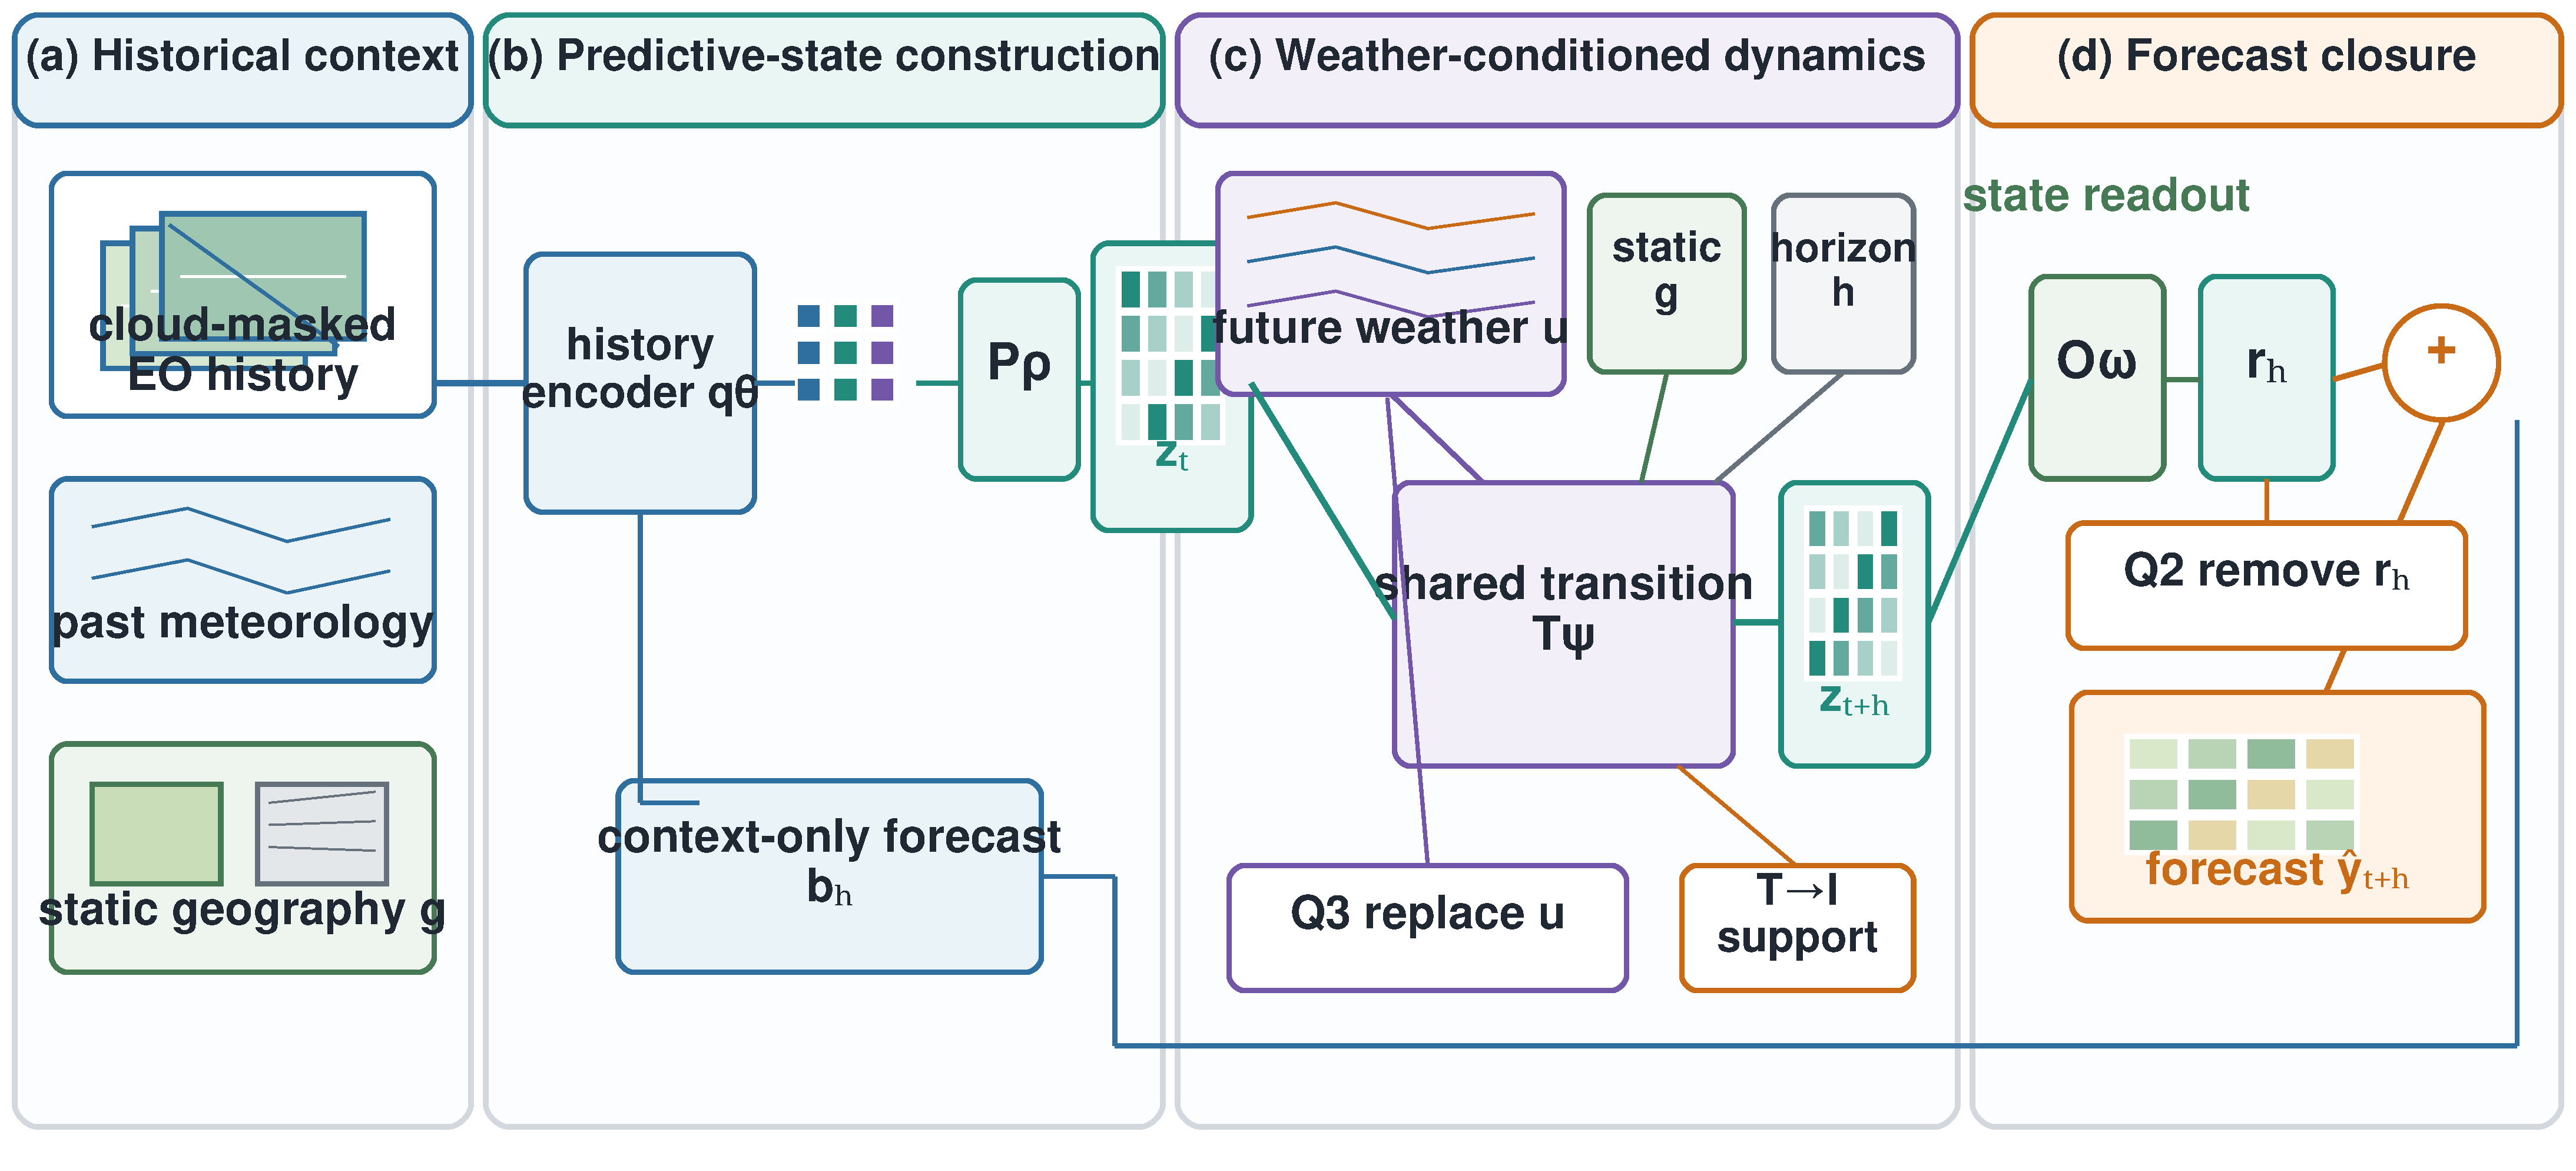
\includegraphics[width=\textwidth]{../paper/figures/terrastate_architecture_fig2.pdf}
\caption{TerraState 详细架构与干预接口}
\end{figure}

云掩膜 EO 历史、过去气象观测和静态地理进入历史编码器 $q_\theta$。上下文 token 一方面产生仅上下文预测 $b_h$，另一方面经 $P_\rho$ 构造预测状态 $z_t$。未来天气只在共享天气条件转移 $T_\psi$ 处进入模型，并与静态地理和 查询时距共同推进状态。$O_\omega$ 将推进后的状态读成 $r_h$，再按 $\widehat y_{t+h}=b_h+r_h$ 闭合最终预测。虚线端口表示训练后的干预：Q2 以 移除 $r_h$ 为状态贡献主检验，$T\rightarrow I$ 仅作辅助；Q3 只替换未来天气 输入。图中的图像式方块均为原创架构示意，不是定性实验结果。

\textbf{数据与模型选择。} 我们使用 GreenEarthNet \cite{benson2024multimodal}。每个 minicube 包含 30 个五日 Sentinel-2 合成帧，空间大小为 $128\times128$、 地面采样距离为 20 m，并对齐气象、云/质量掩膜与高程。前 10 个合成帧构成 上下文，后 20 个定义预测目标时域。模型只按验证集预测能力选择；Q2、Q3 和 OOD-t 数据均不参与。选定模型在本地可用的 OOD-t 划分上评测一次，共 1,904 个 minicube。由于该本地集合没有包含所有官方划分，本文不把它称为完整 GreenEarthNet 官方协议。

\textbf{目标与指标。} 主目标是同时满足有效性和声明植被土地覆盖范围的像素上的 NDVI。Q1 报告 dataset-level $R^2$ 和 RMSE。Q2 将 dataset-level 官方 $\Delta R^2$ 与逐 minicube 配对效应的均值及 bootstrap 区间分开报告。Q3 在匹配子集上报告 $R^2$、RMSE，以及终点损失增量和地理簇 bootstrap 区间。 所有本地评测使用相同的评分与聚合规则。

\textbf{比较对象。} Published 基线直接誊录 GreenEarthNet/Contextformer 论文的 公开结果并标记为 Reported \cite{benson2024multimodal}；这些方法不在本地复现。 由于尚未建立数据子集与评分协议的精确等价性，TerraState 被放在单独的本地 面板中。因此，本文不在 Published 与 Local 面板之间作严格排名。

\textbf{实现与统计。} TerraState 使用 PVT v2/\allowbreak Contextformer 历史编码器、投影后的 空间状态、公式（4）的共享转移，以及公式（5）的预测闭环。模型包含 7,180,896 个唯一 \texttt{nn.Parameter} 标量：统计包含冻结的 $q$ 骨干，但不包含 buffer、训练期 教师和目标编码器。训练前 80\% 有 1,120,336 个可训练参数，最后 20\% 有 1,910,096 个。每个 minicube 的状态形状为 $[1024,256]$，运行时为 $[1024B,256]$。优化使用 AdamW （$\beta=(0.9,0.999)$、weight decay 为 0），共 40 个 epoch、14,880 次更新， 全局 batch 为 64；前 300 步线性 warmup，随后余弦衰减，并在 1.0 处裁剪梯度。 非 $q$ 分支学习率为 $3\times10^{-5}$，$q$ 参数组只在最后 20\% 使用 $9.9\times10^{-7}$。Q1–Q3 使用同一个选定模型。Q2 的 bootstrap 以 minicube 为配对单位，Q3 主置信区间以地理簇为单位。当前结果来自一次训练，不能证明训练 稳定性。

\subsection*{表 1：Q1 预测表现}

\begin{center}
\small
\begin{tabularx}{\textwidth}{@{}Y Y Y Y@{}}
\toprule
\textbf{方法} & \textbf{来源/协议} & \textbf{$R^2\uparrow$} & \textbf{RMSE $\downarrow$} \\
\midrule
\emph{A. GreenEarthNet OOD-t 公开均值} &  &  &  \\
Climatology & Reported & 0.58 & 0.18 \\
ConvLSTM & Reported & 0.58 & 0.16 \\
PredRNN & Reported & 0.62 & 0.15 \\
Contextformer & Reported & 0.62 & 0.14 \\
\emph{B. TerraState 本地评测} &  &  &  \\
\textbf{TerraState} & Local OOD-t & \textbf{0.569} & \textbf{0.151} \\
\bottomrule
\end{tabularx}
\end{center}

\textbf{表注。} Table 1 报告时间偏移下的植被预测表现。为压缩篇幅，Panel A 誊录 Contextformer 原论文 Table 2 的代表性 GreenEarthNet OOD-t 均值并省略 不确定性；Panel B 报告选定 TerraState 模型在 1,904 个本地目标上的结果。 由于精确协议等价性尚未建立，本文不作严格跨面板排名。

\subsection{Q1：时间偏移下的预测能力}

Table 1 的公开面板只提供背景，不构成严格比较。TerraState 在 1,904 个本地 OOD-t minicube 上达到 $R^2=0.56935$、RMSE $=0.15059$。这支持 “模型在时间偏移下保留有效预测能力”这一限定的 Q1 主张。

\subsection{Q2：承载预测的状态}

Q2 隔离推进后状态所承载的贡献。主干预移除 $r_h$，精确恢复仅上下文预测；辅助干预则把 $T_\psi$ 替换为恒等映射。

\subsection*{表 2：状态路径与转移干预}

\begin{center}
\small
\begin{tabularx}{\textwidth}{@{}Y Y Y Y@{}}
\toprule
\textbf{划分} & \textbf{干预} & \textbf{$R^2$：完整 $\rightarrow$ 干预后} & \textbf{官方 $\Delta R^2$} \\
\midrule
Validation & 状态贡献切除 & $0.4973\rightarrow0.4861$ & 0.01121 \\
 & 配对效应 & 0.01616；95\% CI $[0.00643,0.02590]$ &  \\
Validation & $T=\mathrm{Id}$ & $0.4973\rightarrow0.4854$ & 0.01191 \\
 & 配对效应 & 0.01742；95\% CI $[0.00782,0.02696]$ &  \\
OOD-t & 状态贡献切除 & $0.5693\rightarrow0.5494$ & 0.01997 \\
 & 配对效应 & 0.02200；95\% CI $[0.01422,0.03018]$ &  \\
OOD-t & $T=\mathrm{Id}$ & $0.5693\rightarrow0.5477$ & 0.02169 \\
 & 配对效应 & 0.02402；95\% CI $[0.01609,0.03217]$ &  \\
\bottomrule
\end{tabularx}
\end{center}

\textbf{表注。} Table 2 在同一个选定 TerraState 模型上报告 Q2 状态路径与转移干预。官方 $\Delta R^2$ 是 dataset-level 官方指标之差；配对效应是逐 minicube 差异的均值及其 paired-bootstrap 95\% 区间，二者是不同统计量，因此分开报告。状态贡献切除是主干预并恢复仅上下文预测。由于 $T\rightarrow I$ 可能产生训练分布之外的状态读出输入，它只支持转移参与预测。

状态贡献切除使验证集和 OOD-t 上的 dataset-level 官方 $R^2$ 分别下降 $0.01121$ 和 $0.01997$。作为另一统计量，逐 minicube 配对效应均值分别为 $0.01616$ （95\% CI $[0.00643,0.02590]$）和 $0.02200$ （95\% CI $[0.01422,0.03018]$）。两个配对区间都不跨零，因此状态介导路径在两个划分上都承载预测。恒等转移结果方向一致，但由于该干预改变了状态读出的输入分布，只能辅助说明转移参与预测。我们没有直接统计比较两个主效应，因此不主张状态贡献在 OOD-t 上变得更强。

\subsection{Q3：天气驱动响应}

Q3 检验预测对未来天气的响应保真度。在预声明极端天气分层的 84 个匹配样本对上，真实未来天气分别与 matched-donor weather 和归一化均值天气比较。

\subsection*{表 3：天气干预}

\begin{center}
\small
\begin{tabularx}{\textwidth}{@{}Y Y Y@{}}
\toprule
\textbf{未来天气输入} & \textbf{$R^2$ / RMSE} & \textbf{$\Delta$Loss［地理簇 95\% CI］} \\
\midrule
真实天气 & 0.6254 / 0.1492 & reference \\
Matched-donor weather & 0.5893 / 0.1584 & 0.00257 $[0.00112,0.00399]$ \\
归一化均值天气 & 0.5430 / 0.1971 & 0.01126 $[0.00547,0.01708]$ \\
\bottomrule
\end{tabularx}
\end{center}

\textbf{表注。} Table 3 报告 84 对极端天气匹配样本上的天气干预。$\Delta$Loss 表示用指定对照替换真实未来天气后终点损失的增量；正值表示真实天气更好。这里的 actual、matched-donor 和 normalized-mean 分数只针对 Q3 子集，并不是 Table 1 中完整 OOD-t 的 Q1 结果。

真实未来天气相较两个对照都产生更低的终点损失。Matched-donor 对照的配对损失增量为 $0.00257$，地理簇 95\% CI 为 $[0.00112,0.00399]$；归一化均值天气的增量为 $0.01126$，95\% CI 为 $[0.00547,0.01708]$。真实天气更准确地预测观察终点，满足“不能只看状态移动” 的天气响应保真度判据。探索性的 hot-dry 交互为 $0.00044$，置信区间 $[-0.00216,0.00320]$ 跨零，因此本文不主张极端条件特异增强。

\subsection*{图 3 状态说明（非正文）}

\begin{itemize}
\item 未来 Figure 3 必须使用 Q2 \textbf{paired effect mean} 及其 paired CI，并使用 Q3 损失增量及地理簇 CI。不得把 official $\Delta R^2$ 点估计与 paired CI 混画；定性面板还需要固定 EO 样本与统一色标。
\end{itemize}

\section{局限性与适用范围}

TerraState 学到的是由卫星历史和所提供气象约束的未来预测表示，而不是完整物理地表状态。实验把未来天气作为已观测的外生输入；改用业务天气预报时，性能可能降低。

匹配天气与对照天气的差异衡量条件预测保真度，不构成因果识别或反事实正确性。 Hot-dry 交互区间跨零，因此证据不支持极端条件特异增强。预测闭环只支持 “状态介导分支承载可测预测增量”这一主张；它不能证明所有准确输出成分或 $z_t$ 中的全部历史信息都不可替代。

结果来自一次选定训练和一个 OOD-t 轨道，不能证明训练稳定性或跨数据集泛化。公开结果与冻结本地评测不能建立严格跨实现排名。光学目标还会受到云筛选与土壤湿度、灌溉和植被类型等未观测变量影响。时间组合仍未作为核心经验主张得到验证。

\section{结论}

TerraState 使 EO 世界模型的预测状态能够在预测路径内部直接接受检验。模型保留 了有效的 OOD-t 预测能力；状态介导贡献在验证集和 OOD-t 上均为正，且配对区间 不跨零；真实未来天气比 matched-donor weather 或归一化均值天气更准确地预测 终点。这些结果支持一个承载预测、响应天气的预测状态，同时把因果解释、极端 条件特异增强、时间组合与更广泛泛化留作开放问题。


\clearpage
\appendix
\section{中文审阅导航（非投稿正文）}

\subsection{建议优先审核的五个问题}

\begin{enumerate}
\item \textbf{贡献是否成立：} “让预测状态进入预测闭环，并在同一模型上检验其状态贡献和天气响应”是否构成清楚的方法贡献？
\item \textbf{方法是否容易理解：} 公式（1）至（5）能否让读者明确区分历史上下文、共享转移、状态读出和仅上下文预测？
\item \textbf{训练是否可信：} 公式（6）至（9）的真实目标、冻结教师和未来状态锚定是否层级清楚，是否会被误解成 Q2 的替代证据？
\item \textbf{证据是否支持主张：} Q1 只支持有效预测能力；Q2 支持状态路径承载预测；Q3 只支持预测行为依赖所提供天气，不支持因果正确性。
\item \textbf{限制是否足够诚实：} 一次训练、单个 OOD-t 轨道、不同协议的公开比较，以及 hot-dry 未通过是否都得到充分披露？
\end{enumerate}

\subsection{核心 claim–evidence 对照}

\begin{center}
\small
\begin{tabularx}{\textwidth}{@{}Y Y Y@{}}
\toprule
\textbf{核心主张} & \textbf{直接证据} & \textbf{当前状态} \\
\midrule
TerraState 保留有效预测能力 & OOD-t $R^2=0.56935$、RMSE $=0.15059$ & 支持 \\
状态介导路径承载预测 & Validation/OOD-t 状态切除 official $\Delta R^2>0$，paired CI 均高于零 & 支持 \\
共享转移参与预测 & $T\rightarrow I$ 的结果方向一致 & 辅助支持，存在读出分布变化 \\
预测行为依赖未来天气 & 真实天气相较 matched-donor/normalized-mean 的损失更低，CI 均高于零 & 支持 \\
极端热旱条件下增强更强 & hot-dry interaction CI 跨零 & 不支持，正文已明确降级 \\
因果或反事实天气模拟正确 & 当前干预不能识别因果 & 不主张 \\
时间组合一致或非退化 & Q4 不是核心结果 & 不主张 \\
\bottomrule
\end{tabularx}
\end{center}

\clearpage
\bibliographystyle{plainnat}
\bibliography{../paper/references}
\end{document}
